\documentclass{beamer}
\usepackage{tikz}
\usepackage{float}
\usepackage{caption}
\usetikzlibrary{shapes,shapes.geometric,arrows,fit,calc,positioning,automata}
\tikzset{elliptic state/.style={draw,ellipse}}

\def\Tiny{\fontsize{5pt}{5pt} \selectfont}

\newfloat{program}{thp}{lop}
\floatname{program}{Program}

\newfloat{automaton}{thp}{lop}
\floatname{automaton}{Automaton}

\usetheme{default}
\definecolor{light-gray}{gray}{0.80}

\newcommand{\newframe}[3]{
\begin{frame}
\frametitle{#1}
\framesubtitle{#2}
#3
\end{frame}
}

\newcommand{\introslide}[2]{
\newframe{Wireless Sensor Networks}{#1}{
   #2
   }
}

\begin{document}
\title{Wireless Sensor Networks}
\author[Prakhar Banga, Vineet Hingorani]{
\begin{tabular}{cc}
Prakhar Banga & Vineet Hingorani\\
\texttt{prakban@iitk.ac.in} & \texttt{viner@iitk.ac.in}
\end{tabular}\\[0.3cm]
Prof. Sumit Ganguly\\
\texttt{sganguly@iitk.ac.in}\\[0.3cm]
Dept. of CSE, I.I.T. Kanpur
}

\newframe{}{}{
   \titlepage
}

\newframe{Sensors}{}{
\begin{itemize}
   \item<2-> A device with sensing capability:
   \begin{itemize}
      \item<3-> Thermometer\uncover<4->{(Temperature)}
      \item<5-> Hygrometer\uncover<6->{(Humidity)}
      \item<7-> Microphone\uncover<8->{(Sound)}
   \end{itemize}
   \item<9-> Wireless sensor nodes contain:
   \begin{itemize}
      \item<10-> A sensor/sensors
      \item<11-> Microprocessor
      \item<12-> Storage
      \item<13-> Wirless module
   \end{itemize}
\end{itemize}
}

\introslide{}{
   \begin{itemize}
      \item<2-> Networks built for sensor applications
      \item<3-> Consist of sensor nodes and gateway nodes
      \item<4-> Nodes may/may not be capable of computations
      \item<5-> Usually used for monitoring
      \item<6-> Examples:
      \begin{itemize}
         \item<7-> Forest Fire detection
         \item<8-> Activity monitoring(Security)
         \item<9-> GPS tracking
         \item<10-> Plant health monitoring
         \item<11-> ...and various others
      \end{itemize}
   \end{itemize}
}

\introslide{Differences with ad-hoc networks} {
\begin{itemize}
   \item<2-> Dense deployment
   \item<3-> Large number of nodes
   \item<4-> Unreliable nodes
   \item<5-> Broadcast/Multicast paradigm
   \item<6-> Limited node capability
   \item<7-> Addressing issues
\end{itemize}
}

\introslide{Deployment And Maintanence}{
   \uncover<2->{Current state-of-art:}
   \begin{itemize}
      \item<3-> System development from scratch
      \item<4-> Nodes are programmed individually
      \item<5-> Installed at various locations
      \item<6-> Small changes done manually:
      \begin{itemize}
         \item<7-> Changes in logical structure of network
         \item<8-> Reprogramming of nodes
      \end{itemize}
   \end{itemize}
}

\newframe{Problem Statement}{}{
\uncover<2->{Designing a general framework:}
\begin{itemize}
   \item<3-> General system architecture to suit all needs
   \item<4-> Highly flexible, supports remote changes
   \item<5-> Should be lightweight, secure, reliable, fault-tolerant
   \item<6-> Analogous to systemization of database(1970s)
\end{itemize}
}

\newframe{Problem Statement}{Constraints}{
\uncover<2->{Hardware constraints:}
\begin{itemize}
   \item<3-> Costs involved
   \item<4-> Energy consumption
   \item<5-> Communication range
   \item<6-> Data transfer rate
   \item<7-> Limited storage 
   \item<8-> Processing power
\end{itemize}
}

\newframe{Problem Statement}{Constraints}{
\uncover<2->{Design constraints:}
\begin{itemize}
   \item<3-> Application dependent:
   \begin{itemize}
      \item<4->{Mobile vs. fixed nodes}
      \item<5->{Level of security}
      \item<6->{Central vs. Distributed processing}
   \end{itemize}
   \item<7-> Topology dependent:
   \begin{itemize}
      \item<8->{No. of sensor vs. gateway nodes}
      \item<9->{Personal area vs. Wide area}
   \end{itemize}
\end{itemize}
}

\newframe{Related Work}{}{
\begin{itemize}
   \item<2-> Use of TinyOS is prevalent
   \item<3-> Virtual machine code as programs
   \item<4-> CSMA and TDMA as MAC Protocols
   \item<5-> Flooding the network with packets
   \item<6-> Most of these use Berkeley Motes
\end{itemize}
\uncover<7-> {Disadvantages:}
\begin{itemize}
   \item<8-> Hardware Costs suffer a lot
   \item<9-> TinyOS is really not `tiny'
   \item<10-> No capability to map virtual code to binary
   \item<11-> Speed of networking suffers
\end{itemize}
}

\newframe{Various Issues}{}{
\begin{itemize}
   \item<2-> Programming Paradigm
   \begin{itemize}
      \item<3-> Programming Interface
      \item<4-> Version Control
      \item<5-> Dissemination/Acquisition
   \end{itemize}
   \item<6-> Networking
   \begin{itemize}
      \item<7-> Scheduling
      \item<8-> Addressing
   \end{itemize}
   \item<9-> OS
   \begin{itemize}
      \item<10-> Very lightweight
      \item<11-> Modular for required changes
      \item<12-> Layered model
   \end{itemize}
\end{itemize}
}

\newframe{Proposed Architecture}{Stack Model}{
%\begin{itemize}
   \uncover<2-> {
   \begin{center}
      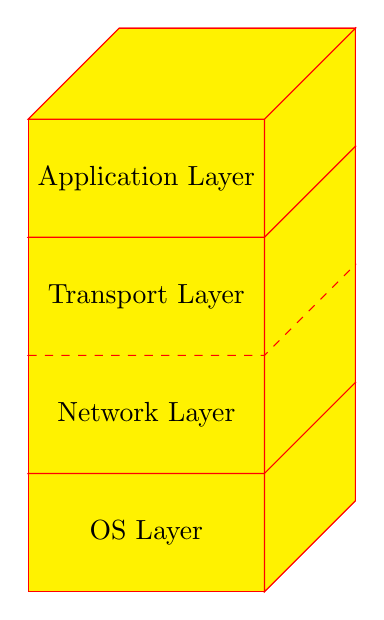
\begin{tikzpicture}
         \pgfmathsetmacro{\cubex}{3}
         \pgfmathsetmacro{\eachcubey}{1.5}
         \pgfmathsetmacro{\cubez}{3}
         \uncover<2-5>{\draw[red,fill=yellow] (0,-3*\eachcubey,0) -- ++(-\cubex,0,0) -- ++(0,-\eachcubey,0) -- ++(\cubex,0,0) -- cycle;}
         \uncover<2-5>{\draw[red,fill=yellow] (0,-3*\eachcubey,0) -- ++(0,0,-\cubez) -- ++(0,-\eachcubey,0) -- ++(0,0,\cubez) -- cycle;}
         \uncover<2-5>{\draw[red,fill=yellow] (0,-3*\eachcubey,0) -- ++(-\cubex,0,0) -- ++(0,0,-\cubez) -- ++(\cubex,0,0) -- cycle;}

         \uncover<3-5>{\draw[red,fill=yellow] (0,-2*\eachcubey,0) -- ++(-\cubex,0,0) -- ++(0,-\eachcubey,0) -- ++(\cubex,0,0) -- cycle;}
         \uncover<3-5>{\draw[red,fill=yellow] (0,-2*\eachcubey,0) -- ++(0,0,-\cubez) -- ++(0,-\eachcubey,0) -- ++(0,0,\cubez) -- cycle;}
         \uncover<3-5>{\draw[red,fill=yellow] (0,-2*\eachcubey,0) -- ++(-\cubex,0,0) -- ++(0,0,-\cubez) -- ++(\cubex,0,0) -- cycle;}

         \uncover<4-5>{\draw[red,fill=yellow] (0,-\eachcubey,0) -- ++(-\cubex,0,0) -- ++(0,-\eachcubey,0) -- ++(\cubex,0,0) -- cycle;}
         \uncover<4-5>{\draw[red,fill=yellow] (0,-\eachcubey,0) -- ++(0,0,-\cubez) -- ++(0,-\eachcubey,0) -- ++(0,0,\cubez) -- cycle;}
         \uncover<4-5>{\draw[red,fill=yellow] (0,-\eachcubey,0) -- ++(-\cubex,0,0) -- ++(0,0,-\cubez) -- ++(\cubex,0,0) -- cycle;}

         \uncover<5-5>{\draw[red,fill=yellow] (0,0,0) -- ++(-\cubex,0,0) -- ++(0,-\eachcubey,0) -- ++(\cubex,0,0) -- cycle;}
         \uncover<5-5>{\draw[red,fill=yellow] (0,0,0) -- ++(0,0,-\cubez) -- ++(0,-\eachcubey,0) -- ++(0,0,\cubez) -- cycle;}
         \uncover<5-5>{\draw[red,fill=yellow] (0,0,0) -- ++(-\cubex,0,0) -- ++(0,0,-\cubez) -- ++(\cubex,0,0) -- cycle;}

         \uncover<2-5>{\node[draw=none] at (-0.5*\cubex,-3.5*\eachcubey,0) {OS Layer};}
         \uncover<3-5>{\node[draw=none] at (-0.5*\cubex,-2.5*\eachcubey,0) {Network Layer};}
         \uncover<4-5>{\node[draw=none] at (-0.5*\cubex,-1.5*\eachcubey,0) {Transport Layer};}
         \uncover<5-5>{\node[draw=none] at (-0.5*\cubex,-0.5*\eachcubey,0) {Application Layer};}

         \uncover<6->{
         \draw[red,fill=yellow] (0,0,0) -- ++(-\cubex,0,0) -- ++(0,-4*\eachcubey,0) -- ++(\cubex,0,0) -- cycle;
         \draw[red,fill=yellow] (0,0,0) -- ++(0,0,-\cubez) -- ++(0,-4*\eachcubey,0) -- ++(0,0,\cubez) -- cycle;
         \draw[red,fill=yellow] (0,0,0) -- ++(-\cubex,0,0) -- ++(0,0,-\cubez) -- ++(\cubex,0,0) -- cycle;
         
         \draw[red,fill=none] (-\cubex,-\eachcubey,0) -- ++(\cubex, 0, 0) -- ++(0, 0, -\cubez);
         \draw[red,fill=none,dashed] (-\cubex,-2*\eachcubey,0) -- ++(\cubex, 0, 0) -- ++(0, 0, -\cubez);
         \draw[red,fill=none] (-\cubex,-3*\eachcubey,0) -- ++(\cubex, 0, 0) -- ++(0, 0, -\cubez);

         \node[draw=none] at (-0.5*\cubex,-3.5*\eachcubey,0) {OS Layer};
         \node[draw=none] at (-0.5*\cubex,-2.5*\eachcubey,0) {Network Layer};
         \node[draw=none] at (-0.5*\cubex,-1.5*\eachcubey,0) {Transport Layer};
         \node[draw=none] at (-0.5*\cubex,-0.5*\eachcubey,0) {Application Layer};
         }
      \end{tikzpicture}
   }
   \end{center}
%\end{itemize}
}

\newframe{Proposed Architecture}{Hierachical Control System}{
\begin{itemize}
   \item<2->n layers of nodes
   \uncover<3->{
      \begin{center}
      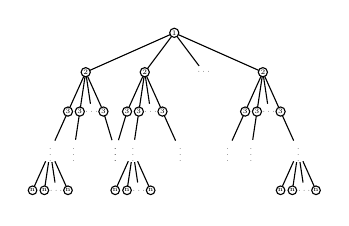
\begin{tikzpicture}[level 1/.style={sibling distance=7.5mm, level distance=5mm},level 2/.style={sibling distance=1.5mm},level 3/.style={sibling distance=1.5mm},level 4/.style={sibling distance=1.5mm},level 5/.style={sibling distance=1.5mm},
      every node/.style={font=\tiny, circle, inner sep=0.7pt, outer sep=0pt, draw, minimum size=0pt, scale=0.5}]
      \node[circle,draw] (a) {1}
      child{ node [circle,draw] (b) {2}
         child{ node [circle,draw] (c) {3} 
            child{ node [draw=none] (c2) {$\vdots$}
               child{ node [circle,draw] (c21) {n} }
               child{ node [circle,draw] (c22) {n} }
               child{ node [draw=none] (c23) {$\cdots$} }
               child{ node [circle,draw] (c24) {n} }
            }
            child{ node [draw=none] (c1) {} edge from parent[draw=none]}
            child{ node [draw=none] (c3) {} edge from parent[draw=none]}
            child{ node [draw=none] (c4) {} edge from parent[draw=none]}
         }
         child{ node [circle,draw] (d) {3} 
            child{ node [draw=none] {} edge from parent[draw=none]}
            child{ node [draw=none] {$\vdots$} }
            child{ node [draw=none] {} edge from parent[draw=none]}
            child{ node [draw=none] {} edge from parent[draw=none]}
         }
         child{ node [draw=none] (e) {$\cdots$} }
         child{ node [circle,draw] (f) {3} 
            child{ node [draw=none] {} edge from parent[draw=none]}
            child{ node [draw=none] {} edge from parent[draw=none]}
            child{ node [draw=none] {} edge from parent[draw=none]}
            child{ node [draw=none] {$\vdots$} }
            child{ node [draw=none] {} edge from parent[draw=none]}
         }
      }
      child{ node [circle,draw] (g) {2} 
         child{ node [circle,draw] (h) {3} 
            child{ node [draw=none] {} edge from parent[draw=none]}
            child{ node [draw=none] {$\vdots$} }
            child{ node [draw=none] {} edge from parent[draw=none]}
            child{ node [draw=none] {} edge from parent[draw=none]}
            child{ node [draw=none] {} edge from parent[draw=none]}
         }
         child{ node [circle,draw] (i) {3} 
            child{ node [draw=none] (i1) {} edge from parent[draw=none]}
            child{ node [draw=none] (i2) {$\vdots$}
               child{ node [circle,draw] (i21) {n} }
               child{ node [circle,draw] (i22) {n} }
               child{ node [draw=none] (i23) {$\cdots$} }
               child{ node [circle,draw] (i24) {n} }
            }
            child{ node [draw=none] (i3) {} edge from parent[draw=none]}
            child{ node [draw=none] (i4) {} edge from parent[draw=none]}
         }
         child{ node [draw=none] (j) {$\cdots$} }
         child{ node [circle,draw] (k) {3} 
            child{ node [draw=none] {} edge from parent[draw=none]}
            child{ node [draw=none] {} edge from parent[draw=none]}
            child{ node [draw=none] {} edge from parent[draw=none]}
            child{ node [draw=none] {$\vdots$} }
         }
      }
      child{ node [draw=none] (l) {$\cdots$} }
      child{ node [circle,draw] (m) {2} 
         child{ node [circle,draw](n){3} 
            child{ node [draw=none] {$\vdots$} }
            child{ node [draw=none] {} edge from parent[draw=none]}
            child{ node [draw=none] {} edge from parent[draw=none]}
            child{ node [draw=none] {} edge from parent[draw=none]}
         }
         child{ node [circle,draw](o){3} 
            child{ node [draw=none] {} edge from parent[draw=none]}
            child{ node [draw=none] {$\vdots$} }
            child{ node [draw=none] {} edge from parent[draw=none]}
            child{ node [draw=none] {} edge from parent[draw=none]}
         }
         child{ node [draw=none] (p){$\cdots$} }
         child{ node [circle,draw](q){3} 
            child{ node [draw=none] (q1) {} edge from parent[draw=none]}
            child{ node [draw=none] (q2) {} edge from parent[draw=none]}
            child{ node [draw=none] (q3) {} edge from parent[draw=none]}
            child{ node [draw=none] (q4) {$\vdots$}
               child{ node [circle,draw] (q41) {n} }
               child{ node [circle,draw] (q42) {n} }
               child{ node [draw=none] (q43) {$\cdots$} }
               child{ node [circle,draw] (q44) {n} }
            }
         }
      }
      ;
      \end{tikzpicture}
      \end{center}
   }
   \item<4-> Higher layers have greater capabilities than lower nodes
   \item<5-> Each node(except the lowest layer):
   \begin{itemize}
      \item<6-> Assigns `tasks' to its children
      \item<7-> Gathers data from its children
      \item<8-> Processes the gathered data and sends data back to its parent
   \end{itemize}
   \item<9-> The tasks are:
   \begin{itemize}
      \item<10-> Programs in an query-based language
      \item<11-> Aimed at data filtering/aggregation
   \end{itemize}
\end{itemize}
}

\newframe{Proposed Architecture}{Addressing}{
\begin{itemize}
   \item<2-> Assumption: need not address individual nodes
   \item<3-> Application level adressing:
   \begin{itemize}
      \item<4-> Novel Concept of Attribute-Value pairs:\\[0.2cm]
      \tiny{
      \uncover<5->{
         \begin{tabular}{|l|l|}
         \hline
         Attribute & Value \\
         \hline
         A1 & V1 \\
         A2 & V2 \\
         A3 & V3 \\
         \vdots & \vdots \\
         Ak & Vk \\
         \hline
         \end{tabular} \\[0.2cm]
      }}

      \item<6-> Properties used to distribute and diffuse the tasks
   \end{itemize}
   \item<7-> Examples: 
   \begin{tabular}{cc}
      \tiny{
         \uncover<8->{
               \begin{tabular}{|l|l|}
               \hline
               Attribute & Value \\
               \hline
               Floor & 3 \\
               Lab & 1 \\
               Row & 5 \\
               \hline
               \end{tabular}
         }
      } &
      \tiny{
         \uncover<9->{
            \begin{tabular}{|l|l|}
            \hline
            Attribute & Value \\
            \hline
            Animal & Lion \\
            Location & Pond Area \\
            Age of Animal & 4 \\
            \hline
            \end{tabular}
         }
      } \\[0.4cm]
      \uncover<8->{Smart Building} & \uncover<9->{Animal Monitoring} \\
   \end{tabular}
\end{itemize}
}

\newframe{Proposed Architecture}{Mobility}{
\begin{itemize}
   \item<2-> Addressing is a challenge in general mobile WSNs
   \item<3-> Using the addressing scheme proposed:
   \begin{itemize}
      \item<4-> A node can change its value for the attributes
      \item<5-> Signal Strength, GPS, other landmarks can be used to change the Table
   \end{itemize}
   \item<6-> Examples:
   \begin{itemize}
      \item<7-> Based on geographic location properties
   \end{itemize}
   \begin{tabular}{cc}
      \tiny{
         \uncover<8->{
               \begin{tabular}{|l|l|}
               \hline
               Attribute & Value \\
               \hline
               Vehicle & Bus \\
               Sub-agency & Krishna \\
               State & Rajasthan \\
               \hline
               \end{tabular}
         }
      } &
      \tiny{
         \uncover<9->{
            \begin{tabular}{|l|l|}
            \hline
            Attribute & Value \\
            \hline
            Vehicle & Bus \\
            Sub-agency & Krishna \\
            State & Gujarat \\
            \hline
            \end{tabular}
         }
      } \\[0.4cm]
      \uncover<8->{Departed Jaipur} & \uncover<9->{Arriving Himmatnagar} \\
   \end{tabular}
   \begin{itemize}
      \item<10-> Based on node particulars
   \end{itemize}
   \begin{tabular}{cc}
      \tiny{
         \uncover<11->{
               \begin{tabular}{|l|l|}
               \hline
               Attribute & Value \\
               \hline
               Troop & 18-Grenadier \\
               Area & Bunker-4 \\
               Condition & Healthy \\
               \hline
               \end{tabular}
         }
      } &
      \tiny{
         \uncover<12->{
            \begin{tabular}{|l|l|}
            \hline
            Attribute & Value \\
            \hline
            Troop & Gurkha \\
            Area & Fence-8 \\
            Condition & Critical \\
            \hline
            \end{tabular}
         }
      } \\[0.4cm]
      \uncover<11->{Fighting Soldier} & \uncover<12->{Soldier Shot} \\
   \end{tabular}
\end{itemize}
}

\newframe{Proposed Architecture}{Query-Based System}{
   \begin{itemize}
      \item<2-> Each node runs a query on some data \\
      \begin{center}
         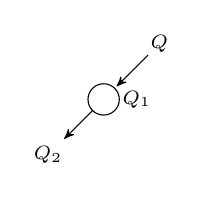
\begin{tikzpicture}[>=stealth',shorten >=1pt,auto,node distance=1cm]
            \tikzstyle{every node}=[font=\scriptsize,inner sep=1pt, minimum size=1pt]
            \tikzset{every state/.style={minimum size=1pt, inner sep=1pt,outer sep=0pt}}
            \uncover<4->{\node[state,draw=none] (n1)      {$Q$};}
            \uncover<3->{\node[state,minimum size=4pt,inner sep=4pt]         (n2) [below left of=n1]  {};}
            \uncover<6->{\node[state,draw=none]         (n3) [below left of=n2] {$Q_{2}$};}
            \uncover<5->{\node[right=0pt of n2] {$Q_{1}$};}
            \uncover<4->{\path[->] (n1) edge [] node {} (n2);}
            \uncover<6->{\path[->] (n2) edge [] node {} (n3);}
            %\node[accepting,state]         (q3) [below of=q1] {$x=[4, \infty], y=5$};
            %\node[accepting,state]         (q4) [below of=q2] {$x=[-\infty, 4), y=3$};


            %\path[->] (S) edge [] node {if x$>$= 4:} (q1)
            %(q1) edge [] node {y:=5}(q3);
            %\path[->] (S) edge [] node {else:} (q2)
            %(q2) edge [] node {y:=3}(q4);
         \end{tikzpicture}
         \uncover<7->{$Q$ = $Q_{1} \circ Q_{2}$}
      \end{center}
      \item<8-> Query splitting based on capabilities.\\
      \uncover<9->{For example,}\\
      \begin{itemize}
      \item 
         \uncover<10->{\small{Sick animal Query}} \\
         \tiny{
            \uncover<11->{$Q$=animal whose body\_temp$>$102;}\\
            \uncover<12->{$Q_2$=animal whose body\_temp$>$102;}\\
            \uncover<13->{$Q_1$=identity;}\\
            \uncover<14->{Lower node filters and sends continuously, upper node resends}\\
            \uncover<15->{ (Instantaneous query)}\\
	 }
      \item
         \uncover<16->{\small{Starving animal Query}} \\
         \tiny{
            \uncover<17->{$Q$=animal id who ate 1 day before;}\\
            \uncover<18->{$Q_2$=send eating animal's id and corresponding time;}\\
            \uncover<19->{$Q_1$=store animal's last eating time and filter for sending;}\\
            \uncover<20->{Lower node sends all data continuously, upper node stores and filters}\\
            \uncover<21->{ (Historical query)}\\
         }
      \end{itemize}
      \item<22-> Novel concept of query composition with data aggregation
   \end{itemize}
}

\newframe{Emergent Systems}{}{
\uncover<2->{A kind of intelligence needed where:}
\begin{itemize}
   \item<3-> Individual nodes perform simple tasks
   \item<4-> Multiple nodes interact to perform complex tasks
\end{itemize}
\uncover<5->{Emergence}\uncover<6->{: Complex systems arising out of a lot of simple interactions}
}

\newframe{Transport Layer}{Challenges}{
\begin{itemize}
   \item<2-> Impact of Re-estimation of Route:
   \begin{itemize}
      \item<3-> Routes can break due to mobility, node failure, etc.
      \item<4-> Throughput reduces after every route breakage
   \end{itemize}
   \item<4-> Frequent Congestion
   \item<5-> High Latency
   \item<6-> Energy efficient reliability and full utilization of resources
\end{itemize}
}

\newframe{Transport Layer}{Approaches and Improvements}{
\uncover<2->{Reliability vital for commercial/enterprise applications}
\begin{itemize}
   \item<3-> Dual Mode operation with Transport Layer enabled or disabled
   \item<4-> TCP: Though time-tested, a very heavy weight protocol
   \item<5-> Protocol needed for wired-cum-wireless networks
   \item<6-> Split TCP with improvements:
   \begin{itemize}
      \item<7-> Performance gain through gateways acting as proxy
      \item<8-> Congestion Control handled by using Buffer at the proxy
   \end{itemize}
   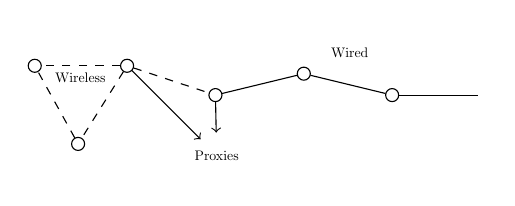
\begin{tikzpicture}
   [every node/.style={scale=0.5}]
   \node[draw, circle] (n1) {};
   \node[draw, circle,left=1cm of n1] (n2) {};
   \node[draw, circle,below left=0.87cm and 0.5cm of n1] (n3) {};
   \node[draw, circle,below right=0.25cm and 1cm  of n1] (n4) {};
   \node[draw, circle,above right=0.15cm and 1cm of n4] (n5) {};
   \node[draw, circle,below right=0.15cm and 1cm of n5] (n6) {};
   \node[draw=none, circle,above left=-0.5cm and 0.25cm of n1] () {Wireless};
   \node[draw=none, circle,above left=0.25cm and 0.25cm of n6] () {Wired};
   \node[draw=none, circle,below right=0.5cm and -0.25cm of n4,inner sep=0pt, minimum size=2pt] (p) {Proxies};
   \node[draw=none, right=1cm of n6] (n7) {};
   \path[dashed] (n1) edge (n2) edge (n3);
   \path[dashed] (n3) edge (n2);
   \path[dashed] (n1) edge (n4);
   \path[-] (n4) edge (n5);
   \path[-] (n5) edge (n6); 
   \path[-] (n6) edge (n7);
   \path[->] (n1) edge (p);
   \path[->] (n4) edge (p);
   \end{tikzpicture}
   \item<9-> End-to-end approach:
   \begin{itemize}
      \item<10-> Deal with losses using Selective ACKs
      \item<11-> Cumulative ACK(sequence number of nth contagious block)
   \end{itemize}
\end{itemize}
}

% \newframe{Refrences}{}{
% 	[1] A Survey of Transport Layer Protocols for Wireless Sensor Networks, International Journal of Computer Applications (0975 - 8887) Volume 33 No 1, November 2011\\
% 	[2] en.wikipedia.org/wiki/Emergence\\
% 	[3] Inc. Crossbow Technology. Mote in-network programming user reference 2003\\
% 	[4] Qiang Wang, Yaoyao Zhu, and Liang Cheng. Reprogramming wireless sensor networks: Challenges and approaches. IEEE Network, 2006\\
% 	[5] Philip Levis and David Culler. The fire-cracker protocol, 2004\\
% 	[6] Sandeep S. Kulkarni and Limin Wang. Mnp: Multihop network reprogramming service for sensor networks. In Proceedings of the 25th International Conference on Distributed Computing Systems ICDCS, pages 7-16, 2005
% }

%\newframe{Transport Layer}{}{}

\end{document}
